\documentclass{article}
\usepackage[utf8]{inputenc}
\usepackage{mathtools}
\usepackage{amssymb}
\usepackage{amsthm}
\usepackage{tcolorbox}
\usepackage{xcolor}
\usepackage{graphicx}
\usepackage{subcaption}

\usepackage{bm}
\newcommand{\vect}[1]{\boldsymbol{\mathbf{#1}}}


% units
\newcommand{\unitLength}{{\mathcal L}}
\newcommand{\unitTime}{{\mathcal T}}

\usepackage{geometry}
\newgeometry{
	left=1.5cm, right=1cm, top=1cm, bottom=1cm,
	includefoot, heightrounded
}

\usepackage{hyperref}
\hypersetup{
	colorlinks=true,
	linkcolor=blue,
	filecolor=magenta,      
	urlcolor=cyan,
}


\let\pa\partial
\let\ep\varepsilon
\newcommand{\R}{\mathbb R}
\newcommand{\bA}{\mathbf A}
\newcommand{\bB}{\mathbf B}
\newcommand{\bC}{\mathbf C}
\newcommand{\bD}{\mathbf D}
\newcommand{\bE}{\mathbf E}
\newcommand{\bH}{\mathbf H}
\newcommand{\bI}{\mathbf I}
\newcommand{\bJ}{\mathbf J}
\newcommand{\bP}{\mathbf P}
\newcommand{\bK}{\mathbf K}
\newcommand{\bM}{\mathbf M}
\newcommand{\bQ}{\mathbf Q}
\newcommand{\bS}{\mathbf S}
\newcommand{\cV}{\mathcal{V}_{\rm div}}
\newcommand{\bV}{\mathbf V}
\newcommand{\ga}{\gamma}
\newcommand{\ba}{\mathbf a}
\newcommand{\bb}{\mathbf b}
\newcommand{\bg}{\mathbf g}
\newcommand{\bj}{\mathbf j}
\newcommand{\blf}{\mathbf f}
\newcommand{\bn}{\mathbf n}
\newcommand{\be}{\mathbf e}
\newcommand{\bp}{\mathbf p}
\newcommand{\br}{\mathbf r}
\newcommand{\bs}{\mathbf s}
\newcommand{\bT}{\mathbf T}
\newcommand{\bu}{\mathbf u}
\newcommand{\bU}{\mathbf U}
\newcommand{\bv}{\mathbf v}
\newcommand{\bw}{\mathbf w}
\newcommand{\bW}{\mathbf W}
\newcommand{\bx}{\mathbf x}
\newcommand{\by}{\mathbf y}
\newcommand{\bz}{\mathbf z}
\newcommand{\bbf}{\mathbf f}
\newcommand{\A}{\mathcal A}
\newcommand{\F}{\mathcal F}
\newcommand{\G}{\mathcal G}
\newcommand{\I}{\mathcal I}
\newcommand{\K}{\mathcal K}
\newcommand{\M}{\mathcal M}
\newcommand{\N}{\mathcal N}
\newcommand{\Q}{\mathcal Q}
\newcommand{\J}{\mathcal J}
\newcommand{\T}{\mathcal T}
\newcommand{\V}{\mathcal V}
\newcommand{\Div}{\mathop{\rm div}}
\newcommand{\divG}{{\mathop{\,\rm div}}_{\Gamma}}
\newcommand{\gradG}{\nabla_{\Gamma}}
\newcommand{\nablaG}{\nabla_{\Gamma}}
\newcommand{\laplG}{\Delta_{\Gamma}}
\newcommand{\cH}{\mathcal H}
\newcommand{\cD}{\mathcal D}
\newcommand{\cF}{\mathcal F}
\newcommand{\cE}{\mathcal E}
\newcommand{\cO}{\mathcal O}
\newcommand{\cT}{\mathcal T}
\newcommand{\cP}{\mathcal P}
\newcommand{\cR}{\mathcal R}
\newcommand{\cS}{\mathcal S}
\newcommand{\cL}{\mathcal L}
\newcommand{\rr}{\mathbb{R}}
\newcommand{\cc}{\mathbb{C}}
\newcommand{\kk}{\mathbb{K}}
\newcommand{\nn}{\mathbb{N}}
\newcommand{\dd}{\,d}
\newcommand{\zz}{\mathbb{Z}}
\newcommand{\Gs}{\mathcal{S}} %{\Gamma_\ast}
\newcommand{\OGamma}{\Omega^\Gamma_h}
\newcommand{\tA}{\widetilde{\mathcal A}}
%\newcommand{\Gsn}{{\Gamma_\ast^n}}
%\newcommand{\normal}{n}
\newcommand{\wn}{w_{\!\perp}}
\newcommand{\ddp}{\partial}
\newcommand{\ati}{\tilde{a}}
\newcommand{\wtang}{\bw_\parallel}
%\newcommand{\grad}{\nabla}
\newcommand{\jumpleft}{[\![}
\newcommand{\jumpright}{]\!]}
\newcommand{\averageleft}{\{\!\!\{}
\newcommand{\averageright}{\}\!\!\}}
\newcommand{\divergence}{\textrm{div}\ \!}
\renewcommand{\div}{\textrm{div}\ \!}
\newcommand{\HSobolev}{H}
\newcommand{\Lzwei}{L^2}
\newcommand{\Rn}{\mathbb{R}^n}
\newcommand{\Rm}{\mathbb{R}^m}
\newcommand{\tr}{{\rm tr}}
%\newcommand{\alert}[1]{{\bf #1}}
\DeclareGraphicsExtensions{.pdf,.eps,.ps,.eps.gz,.ps.gz,.eps.Y}
\def\Fh{\mathcal{F}_h}
\def\Eh{\mathcal{E}_h}
\newcommand{\la}{\left\langle}
\newcommand{\ra}{\right\rangle}
\newcommand{\Yo}{\overset{\circ}{Y}}
\newcommand{\deriv}[2]{\frac{\partial #1}{\partial #2}}
\newcommand{\bsigma}{\boldsymbol{\sigma}}
\newcommand{\DG}{D_\Gamma}
\newcommand{\DGh}{D_{\Gamma_h}}
\newcommand{\bxi}{\mbox{\boldmath$\xi$\unboldmath}}
\def\cl {\nonumber \\}
\def\el {\nonumber }

% differentials
\newcommand*\diff{\mathop{}\!\mathrm{d}}
\newcommand*\Diff[1]{\mathop{}\!\mathrm{d^#1}}

\newcommand{\anna}[2][cyan]{\emph{\textcolor{#1}{#2}}}
\newcommand{\MO}[1]{{\color{blue}#1}}
\newcommand{\VY}[1]{{\color{black!50!green}#1}}
\newcommand{\rev}[1]{{\color{red}#1}}

\newtheorem{mydef}{Definition}[section]
\newtheorem{mybem}{Bemerkung}[section]
\newtheorem{assumption}{Assumption}[section]
\newtheorem{mybsp}{Testbeispiel}[section]
\newtheorem{remark}{Remark}[section]
%\newtheorem{proposition}{Proposition}[section
%\newtheorem{corollary}{Corollary}
\def\enorm#1{|\!|\!| #1 |\!|\!|}
%\numberwithin{equation}{section}
%\numberwithin{figure}{section}

\begin{document}
	\tableofcontents
\newpage	
\section{NSCH system on surfaces with kinematic viscosity}
\begin{align}
 \vect P\,\frac{\partial\vect u_T}{\partial t} + \vect P\,(\vect u\cdot\nabla)\vect u_T - \nu\,\vect P\divG(E_s(\vect u_T)) + u_N\,\vect H\,\vect u_T + \nabla_\Gamma p &=   - \frac{\sigma_\gamma \mu \nablaG c}{\epsilon} \quad &\text{on}~\Gamma,  \label{strongform-1} \\
\divG \bu & =0 \quad &\text{on}~\Gamma, \label{strongform-2}\\
 \frac{\partial c}{\partial t} +\bu\cdot\nablaG c-  \frac{1}{\epsilon}\divG \left(M \gradG \mu \right)  &= 0 \quad &\text{on}~\Gamma \label{eq:sys_CH1}, \\
\mu &= f_0' - \epsilon^2 \laplG c \quad &\text{on}~\Gamma. \label{eq:sys_CH2}
\end{align}


System needs to be supplemented with the
definitions of mobility $M$ and free energy per unit surface $f_0$. A possible choice for $M$
is given by $M = M(c) = c(1 - c).$
This mobility is referred to as a degenerate mobility, since it is not strictly positive.
Again, a common choice for $f_0$ is given by $f_0(c) = \frac{\xi}{4} c^2(1 - c)^2,$
where $\xi$ defines the barrier height, i.e. the local maximum at $c = 1/2$ . We set  $\xi = 1$ in our experiments.


\section{Kelvin-Helmhotz instability on a sphere}

Kelvin-Helmholtz instability simulation \textbf{below} is on mesh level $l=5$ with $\epsilon = 10^{-2};$ line tension $\sigma_\gamma = 10^{-3};$ time interval $t\in [0,20]$ with  640 steps;\\
\begin{figure}[h]
	\centering
	\begin{subfigure}[b]{0.15\textwidth}
		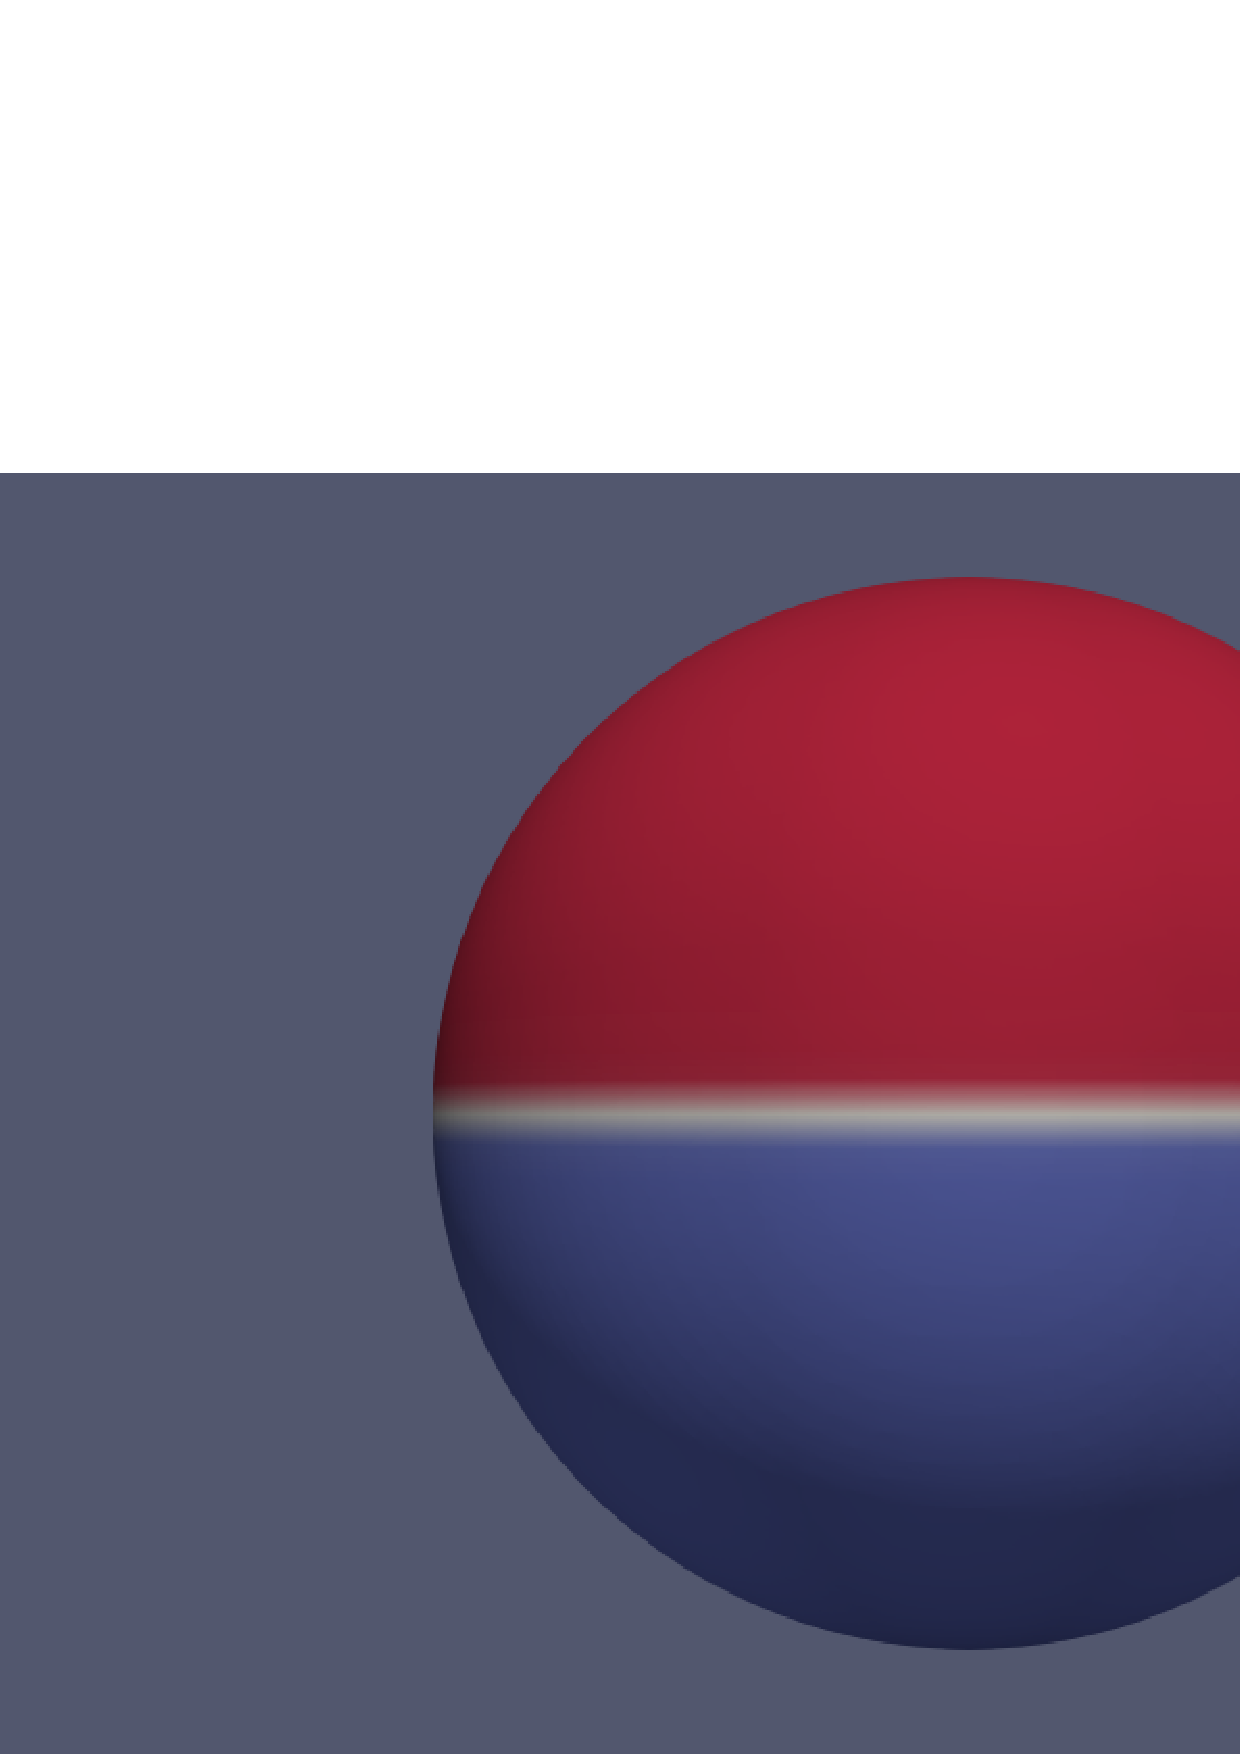
\includegraphics[scale=0.1]{images/c0.png}
		\caption{$t=0$}
	\end{subfigure} 
\begin{subfigure}[b]{0.15\textwidth}
	\includegraphics[scale=0.1]{images/c4375.png}
	\caption{$t=4.375$}
\end{subfigure}
\begin{subfigure}[b]{0.15\textwidth}
	\includegraphics[scale=0.1]{images/c5.png}
	\caption{$t=5$}
\end{subfigure}
\begin{subfigure}[b]{0.15\textwidth}
	\includegraphics[scale=0.1]{images/c625.png}
	\caption{$t=6.25$}
\end{subfigure}
\begin{subfigure}[b]{0.15\textwidth}
	\includegraphics[scale=0.1]{images/c75.png}
	\caption{$t=7.5$}
\end{subfigure}
\begin{subfigure}[b]{0.15\textwidth}
	\includegraphics[scale=0.1]{images/c20.png}
	\caption{$t=20$}
\end{subfigure}
\caption{Snapshots of concentration at given $t$}
\end{figure}
\begin{figure}[h]
	\centering
	\begin{subfigure}[b]{0.15\textwidth}
		\includegraphics[scale=0.1]{images/w0.png}
		\caption{$t=0$}
	\end{subfigure} 
	\begin{subfigure}[b]{0.15\textwidth}
		\includegraphics[scale=0.1]{images/w4375.png}
		\caption{$t=4.375$}
	\end{subfigure}
	\begin{subfigure}[b]{0.15\textwidth}
		\includegraphics[scale=0.1]{images/w5.png}
		\caption{$t=5$}
	\end{subfigure}
	\begin{subfigure}[b]{0.15\textwidth}
		\includegraphics[scale=0.1]{images/w625.png}
		\caption{$t=6.25$}
	\end{subfigure}
	\begin{subfigure}[b]{0.15\textwidth}
		\includegraphics[scale=0.1]{images/w75.png}
		\caption{$t=7.5$}
	\end{subfigure}
	\begin{subfigure}[b]{0.15\textwidth}
		\includegraphics[scale=0.1]{images/w20.png}
		\caption{$t=20$}
	\end{subfigure}
	\caption{Snapshots of concentration at given $t$}
\end{figure}

Click for the animation of \href{https://www.dropbox.com/s/efymgjo6drifeoj/KH-concentration-l5-lt1e3-lmyes-ltyes.avi?dl=0}{concentration} and \href{https://www.dropbox.com/s/mtjzgtt2ec7nuzj/KH-vorticity-l5-lt1e3-lmyes-ltyes.avi?dl=0}{vorticity}.

\subsection{On vortices of KH}
KH simulation forms 4 vortices at around $t=4$, and 3 of 4 are identical fourth one is different. See the figure below(front and back):
\begin{figure}[h]
	\centering
	\begin{subfigure}[b]{0.15\textwidth}
		\includegraphics[scale=0.1]{images/KHvorticity1.png}
		
	\end{subfigure} 
	\begin{subfigure}[b]{0.15\textwidth}
		\includegraphics[scale=0.1]{images/KHvorticity2.png}
		
	\end{subfigure}
	
\end{figure}

\section{Rayleigh-Taylor instability on a torus}

To simulate RT instability we write the NS equation with dynamic viscosity: $\rho(c)=c\rho_0+(1-c)\rho_1$ and viscosity $\eta(c)=c\eta_0+(1-c)\eta_1$

\begin{align}
\rho(c)\vect P\,\frac{\partial\vect u_T}{\partial t} + \rho(c)\vect P\,(\vect u\cdot\nabla)\vect u_T - {\color{red}\frac{1}{Re}}\eta(c)\,\vect P\divG(E_s(\vect u_T)) + u_N\,\vect H\,\vect u_T + \nabla_\Gamma p &=   - \frac{\sigma_\gamma \mu \nablaG c}{\epsilon} + \frac{\rho(c)\textbf{g}}{Fr^2} \quad &\text{on}~\Gamma,  \label{strongform-1} \\
\divG \bu & =0 \quad &\text{on}~\Gamma, \label{strongform-2}\\
\frac{\partial c}{\partial t} +\bu\cdot\nablaG c-  \frac{1}{\epsilon}\divG \left(M \gradG \mu \right)  &= 0 \quad &\text{on}~\Gamma \label{eq:sys_CH1}, \\
\mu &= f_0' - \epsilon^2 \laplG c \quad &\text{on}~\Gamma. \label{eq:sys_CH2}
\end{align}
Parameter used in Kim's \cite{YANG2020113382} paper are: $Re=3000,$ $\rho_0:\rho_1=3:1,$ $\eta_0:\eta_1=1:1$   The surface tension is ignored. $Fr=0.58$

{\color{red} \textbf{Note:}We need , as we discussed in emails, $(\frac{1}{\epsilon}, \epsilon)$ scaling of chemical potential in order, and to fix that we added $\frac{1}{\epsilon}$ scaling to $\divG \left(M \gradG \mu \right)$. However, Kim takes $Pe=\frac{1}{\epsilon}$, which $\epsilon$ scaling instead of $\frac{1}{\epsilon}$.}

\subsection{NSCH for RT from Kim2020\cite{YANG2020113382}}

\begin{align}
\rho(c) \frac{\partial\vect u}{\partial t} + \rho(c)(\vect u\cdot\nabla)\vect u_T - {\color{red}\frac{1}{Re}}\eta(c)\,\divG(E_s(\vect u_T)) + \nabla_\Gamma p &=  \frac{\rho(c)\textbf{g}}{Fr^2} \quad &\text{on}~\Gamma,   \\
\divG \bu & =0 \quad &\text{on}~\Gamma, \\
\frac{\partial c}{\partial t} +\bu\cdot\nablaG c-  \epsilon \divG \left(M \gradG \mu \right)  &= 0 \quad &\text{on}~\Gamma , \\
\mu &= f_0' - \epsilon^2 \laplG c \quad &\text{on}~\Gamma. 
\end{align}

\section{Testing DROPS solver}
\begin{itemize}
	
	
	\item Setting line tension $\sigma_\gamma=0$ makes removes effect of CH on NS, and the solver gives exactly same result as original code.
	
	\item Eliminating convection term from CH removes effect of CH, and solver gives same results as original phase separation codes.
	
	\item Please see the \href{https://www.dropbox.com/sh/bun3sdmbkw9bgax/AAD5kkeIuiPMgwdWsmpdHpFFa?dl=0}{folder} This is test on level 3, the error is getting bigger in each step.
	
	\item Tests with mesh level 6 compute nodes broke two times due write error, probably location run out of memory.\\ \textbf{\textit{ToDo:}} Set output folder to \verb|/scratch/yerbol|. 
\end{itemize}
\newpage

The weak (variational) formulation of the surface Cahn--Hilliard problem \eqref{eq:sys_CH1}--\eqref{eq:sys_CH2}: Find $(c,\mu) \in H^1(\Gamma) \times H^1(\Gamma)$ %(for $\alpha>0$)
such that
\begin{align}
&\int_\Gamma \rho \frac{\partial c}{\partial t} \,v \, ds +{\color{red} \int_\Gamma (\bu\cdot\nablaG c)\, v\, ds} + \int_\Gamma M \gradG \mu \, \gradG v \, ds = 0, \label{eq:sys_CH1_weak} \\
&\int_\Gamma  \mu \,q \, ds - \int_\Gamma \frac{1}{\epsilon}f_0'(c) \,q \, ds - \int_\Gamma \epsilon \gradG c \, \gradG q \, ds = 0, \label{eq:sys_CH2_weak}
\end{align}
for all $ (v,q) \in H^1(\Gamma) \times H^1(\Gamma)$.
%%%%%%%%%%%%%%%%%%%%%%%


At time instance $t^k=k\Delta t$, with time step $\Delta t=\frac{T}{N}$,  $c^k$ denotes the approximation of the order parameter $c(t^k, \bx)$;  similar notation is used for other quantities of interest. Further, we need second order approximation of first and second time derivatives :
 \begin{equation}\label{BDF2}
\left[c\right]_t^{k} =\frac{3c^{k}-4c^{k-1}+c^{k-2}}{2\Delta t},\quad
\left[c\right]_{tt}^{k} =\frac{c^{k+1}-2c^{k}+c^{k-1}}{|\Delta t|^2},
\end{equation}
and linear extrapolation for $f_0'$ at time $t^k$: $\widetilde f_0'(c)^k=2f_0'(c^{k-1})- f_0'(c^{k-2})$. Same notations for differences and extrapolation will be used with other variables.

The semi-implicit stabilized TraceFEM for the Cahn--Hilliard equations
reads: Given $c^{k-1}_h,c^{k-2}_h\in V_h$ and $\mu^{k-1}_h,\mu^{k-2}_h\in V_h$,  find $c_h^k, \mu^k \in V_h$ solving
\begin{equation}\label{eq:CH_FE}
\begin{split}
\int_{\Gamma_h} \rho \left[c_h\right]_t^{k}v_h\,ds    + {\color{red}  \int_{\Gamma_h} (\bu_h^k\cdot\nabla_{\Gamma_h}c_h^k )v_h\,ds }+ \int_{\Gamma_h} M(\widetilde c^k) \nabla_{\Gamma_h}\mu_h^k\cdot\nabla_{\Gamma_h}v_h\,ds +  h \int_{\OGamma} (\bn_h\cdot\nabla \mu_h^k) (\bn_h\cdot\nabla v_h) \, dx\\
%
+\int_{\Gamma_h}\left\{  \mu_h^k - \beta_s|\Delta t|^2\left[{c}_h\right]_{tt}^{k-1} - \widetilde  f'_0( c_h)^{k}\right\}q_h\,ds
- \int_{\Gamma_h} \epsilon^2 \gradG c_h^k \, \gradG q_h \, ds \\ -\epsilon^2 h \int_{\OGamma} ( \bn_h\cdot\nabla c_h^k) (\bn_h\cdot\nabla q_h) \, dx = 0
\end{split}
\end{equation}
for all  $v_h\in V_h$ and $q_h \in V_h$, $k=2,3,\dots,N$. Again, for $k=1$ an obvious first order modification is used and we set $\beta_s=1$.

\begin{equation}\label{eq:CH_FE}
	\begin{split}
		\int_{\Gamma_h} \rho \frac{3c_h^k}{2\Delta t}v_h\,ds    + {\color{red}  \int_{\Gamma_h} (\bu_h^k\cdot\nabla_{\Gamma_h}c_h^k )v_h\,ds }+ \int_{\Gamma_h} M(\widetilde c^k) \nabla_{\Gamma_h}\mu_h^k\cdot\nabla_{\Gamma_h}v_h\,ds +  h \int_{\OGamma} (\bn_h\cdot\nabla \mu_h^k) (\bn_h\cdot\nabla v_h) \, dx\\
		%
		+\int_{\Gamma_h}\left\{  \mu_h^k - \beta_s c_h^k - \widetilde  f'_0( c_h)^{k}\right\}q_h\,ds
		- \int_{\Gamma_h} \epsilon^2 \gradG c_h^k \, \gradG q_h \, ds  -\epsilon^2 h \int_{\OGamma} ( \bn_h\cdot\nabla c_h^k) (\bn_h\cdot\nabla q_h) \, dx \\= \int_{\Gamma_h} \rho \frac{4c_h^{k-1}-c_h^{k-2}}{2\Delta t}v_h\,ds - \int_{\Gamma_h}\left\{\beta_s(2c_h^{k-1}-c_h^{k-2})\right\}q_h\,ds
	\end{split}
\end{equation}

{\color{blue} Expend finite differences $[c_h]_t^{k}$ and $\left[{c}_h\right]_{tt}^{k-1}$ according to \eqref{BDF2} or use implicit Euler for $[c_h]_t^{k}$. Then you will see what terms go to the right-hand side and what constitutes bilinear form on each time step. Find where these bilinear forms are assembled in the code.
This will also  help you to understand for to handle time derivative in the NSE below.}

%%%%%%%%%%%%%%%%%%%%%%%%%%%%%%%%%%%%
\newpage
\section{Navier-Stokes equation}


The surface Stokes problem reads: For a given tangential force vector $\mathbf{f} \in L^2(\Gamma)^3$, i.e. $\mathbf{f}\cdot\bn=0$ holds, and
source term $g\in L^2(\Gamma)$, with $\int_\Gamma g\, ds=0$, find a tangential fluid vector field $\bu:\, \Gamma \to \R^3$, $\bu\cdot\bn =0$, and a surface fluid pressure $p:\, \Gamma \to \R$  such that
\begin{align} %\label{strongform}
  - 2\,\bP \divG (E_s(\bu))+{\color{red}\partial_t\mathbf{u}+ (\nabla_\Gamma \mathbf{u})\mathbf{u}} +\nabla_\Gamma p &=  \blf \quad \text{on}~\Gamma,  \label{strongform-1} \\
  \divG \bu & =0 \quad \text{on}~\Gamma, \label{strongform-2}
\end{align}
{\color{blue} For formal definition of all operators you can see \cite{jankuhn2018incompressible}, where in particular you can find the integration by part identity you are looking for (second equation from he bottom of page 4). It may be helpful to remember that a convolution from a skew-symmetric matrix is zero, that is $A:B=\mbox{tr}(AB^T)=0$, if $B=-B^T$, which implies $E_s(\bu):\nabla_\Gamma(\bu)= E_s(\bu):E_s(\bu)$, since $\nabla_\Gamma(\bu)=E_s(\bu)+\text{Scew Symmetric part}$.\\}

%As for $\mathbf{u}\cdot\nabla_\Gamma \mathbf{u}$, this notation is a bit odd. In the usual planar case, people often write  $(\mathbf{u}\cdot\nabla) \mathbf{u}$, which means componentwise derivative of $\mathbf{u}$ along $\mathbf{u}$, this can be equivalently written as $(\nabla \mathbf{u})\mathbf{u}$  as a multiplication of matrix $(\nabla \mathbf{u})$ with a vector. In the surface case, I would prefer to write  $(\nabla_\Gamma \mathbf{u})\mathbf{u}$, where  $(\nabla_\Gamma \mathbf{u})=\mathbf{P}\nabla \mathbf{u}\mathbf{P}$ is a matrix.

We use the  decomposition of a general vector field into tangential and normal components:
\begin{equation}\label{u_T_N}
\bu = \bu_T + u_N\bn,\quad \bu_T\cdot\bn=0.
\end{equation}
%We remark that further in the text we use both $u_N$ and $\bn\cdot\bu$  to denote the normal component of the velocity $\bu$.

For the weak formulation of the surface Stokes problem \eqref{strongform-1}--\eqref{strongform-2},
we need the vector Sobolev space $\bV\coloneqq  H^1(\Gamma)^3$ equipped with the norm
\begin{equation} \label{H1norm}
	\|\bv\|_{1}\coloneqq \left(\|\bv\|^2_{L^2(\Gamma)} + \|(\nabla\bv^e)\bP\|^2_{L^2(\Gamma)}\right)^{\frac12}
\end{equation}
and its subspace of tangential vector fields
\begin{equation}   \label{defVT}
 \bV_T\coloneqq  \{\, \bv \in \bV\::\: \bv\cdot \bn =0\,\}.
\end{equation}
%Note that $E$ is a closed subspace of $\bV_T$ and $\mbox{dim}(E)\le 3$.
%We define the Hilbert space $\bV_T^0$ as an orthogonal complement of  $E$ in $\bV_T$
%(hence $\bV_T^0 \sim \bV_T/E$).
For $\bv \in \bV$ we will use the orthogonal decomposition into tangential and normal parts
as in \eqref{u_T_N}.
%In what follows, we will need both general and tangential vector fields on $\Gamma$.
%To make the presentation clear, from now on we shall use subscript ${\,}_T$ to label tangential fields.
We define $L_0^2(\Gamma)\coloneqq \{\,p \in L^2(\Gamma)\::\:\int_\Gamma p \diff{s} = 0\,\}$.

Consider the continuous bilinear forms (with $\vect A : \vect B \coloneqq {\rm tr}\big(\vect A \vect B^T\big)$ for  $\vect A, \vect B\in\mathbb{R}^{3\times3}$)
\begin{align}
a(\bu,\bv) &\coloneqq \int_\Gamma (2\,E_s(\bu):E_s(\bv)+{\color{red}\partial_t\mathbf{u}\cdot \bv+ ((\nabla_\Gamma \mathbf{u})\mathbf{u})\cdot \bv}) \diff{s}, \quad \bu,\bv \in \bV, \label{defblfa} \\
b_T(\bv,p) &\coloneqq -\int_\Gamma p\,\divG \bv_T \diff{s},  \quad \bv \in \bV, ~p \in L^2(\Gamma). \label{defblfb}
\end{align}
{\color{blue}
Time derivative should not be in the bilinear form in a finite element method. You first apply finite difference method to $\partial_t\mathbf{u}$ and then keep in the FE bilinear form only terms with $\mathbf{u}^k$. Other terms go to the ``known'' write hand side.
}
Note that in the definition of $b_T(\bv,p)$ only the {tangential} component of $\bv$ is used, i.e., $b_T(\bv,p)=b_T(\bv_T,p)$ for all $\bv \in \bV$, $p\in L^2(\Gamma)$. This property motivates the notation $b_T(\cdot,\cdot)$ instead of $b(\cdot,\cdot)$.
If $p$ is from $H^1(\Gamma)$, then integration by parts yields
\begin{equation}\label{Bform}
b_T(\bv,p)=\int_\Gamma  \bv_T\cdot \gradG p \diff{s} = \int_\Gamma  \bv \cdot \gradG p \diff{s}.
\end{equation}

The weak  formulation of the surface Stokes problem \eqref{strongform-1}--\eqref{strongform-2}
reads: Find %$(\bv_T,p) \in \bV_T^0 \times L_0^2(\Gamma)$ (for $\alpha=0$) or
$(\bu_T,p) \in \bV_T \times L_0^2(\Gamma)$ %(for $\alpha>0$)
such that
\begin{align}
	a(\bu_T,\bv_T) +b_T(\bv_T,p) &=(\blf,\bv_T) \quad \text{for all}~~\bv_T \in \bV_T, \label{Stokesweak1_1} \\
	b_T(\bu_T,q) & = (-g,q) \quad \text{for all}~~q \in L^2(\Gamma). \label{Stokesweak1_2}
\end{align}
%\AZ{Here and further I replaced $g \rightarrow -g$, so everything is consistent with~\eqref{strongform-2} and~\eqref{spsystem}.}
%For $\alpha=0$, the test space $\bV_T$ can be replaced by $\bV_T^0$.
Here $(\cdot,\cdot)$ denotes the $L^2$ scalar product on $\Gamma$.

The bilinear forms that we use in the discretization method contain terms related to algebraic stability and a penalty term. We introduce the following  bilinear forms:
\begin{align}\begin{split}\label{forms}
	A_h(\bu^k, \bv) &\coloneqq
		\int_{\Gamma} (2E_s(\bu^k) : E_s(\bv) + {\color{red}\frac{3}{2\Delta t}\bu^k\cdot \bv+ ((\nabla_\Gamma \mathbf{u}^k)\mathbf{u}^k)\cdot \bv} + \tau\,u_N^k\,v_N)  \diff{s} \\ & ~~~+
		\rho_u \int_{\Omega_h^{\Gamma}} ([\nabla\bu^k]\,\bn)\cdot([\nabla\bv]\,\bn) \diff{\vect x},\\
s_h(p^k,q)& \coloneqq  \rho_p  \int_{\OGamma} (\bn \cdot \nabla p^k)  (\bn \cdot\nabla q) \,  \diff{\vect x},
%b(\bu, q ) &= -\int_{\Gamma} q\,\divG \bu  \diff{s},
\end{split}\end{align}
with the penalty parameter $\tau \geq 0$ and two stabilization parameters $\rho_p  \geq 0$ and $\rho_u \geq 0$. In  practice the (exact) normal $\bn$ used in the bilinear forms $A_h(\cdot,\cdot)$ and $s_h(\cdot,\cdot)$ is replaced by a sufficiently accurate approximation. %In the setting of parametric trace finite element methods, cf. Remark~\ref{Rem1}, such an approximation can easily be computed.

The trace finite element method reads as follows:
Given $ \bu_h^{k-2}, \bu_h^{k-2} \in \bU_h$ find $(\bu_h^k, p_h^k) \in \bU_h \times Q_h$ such that
\begin{equation} \label{discrete}
 \begin{aligned}
  A_h(\bu_h^k,\bv_h) + b_T(\bv_h,p_h^k) & =(\blf+\frac{4\bu^{k-1}-\bu^{k-2}}{2\Delta t},\bv_h) &\quad &\text{for all } \bv_h \in \bU_h, \\
  b_T(\bu_h^k,q_h)-s_h(p_h^k,q_h) & = (-g,q_h) &\quad &\text{for all }q_h \in Q_h.
 \end{aligned}
\end{equation}
We allow the following ranges of  parameters:
\begin{equation} \label{parameters}
\tau= c_\tau h^{-2},\quad \rho_p= c_p h, \quad \rho_u\in [c_u h,C_u h^{-1}].
\end{equation}
Here $h$ is the characteristic mesh size of the background tetrahedral mesh, while
$c_\tau$, $c_p$, $c_u$, $C_u$ are strictly positive constants  independent of $h$ and of how $\Gamma$ cuts through the background mesh. %The optimal value of those constants may depend on problem data such as $\Gamma$, but is independent of $h$ and of how $\Gamma$ cuts through the background mesh.


\newpage
\section{Coupled problem}
\subsection{Strong form}
\begin{align} %\label{strongform}
- 2\,\bP \divG (E_s(\bu))+{\color{red}\partial_t\mathbf{u}+ (\nabla_\Gamma \mathbf{u})\mathbf{u}} +\nabla_\Gamma p &=   - \sigma_\gamma \mu \nablaG c \quad \text{on}~\Gamma,  \label{strongform-1} \\
\divG \bu & =0 \quad \text{on}~\Gamma, \label{strongform-2}\\
\rho \frac{\partial c}{\partial t} +\bu\cdot\nablaG c-  \divG \left(M \gradG \mu \right)  &= 0 \quad \text{on}~\Gamma \label{eq:sys_CH1}, \\
\mu &= f_0' - \epsilon^2 \laplG c \quad \text{on}~\Gamma. \label{eq:sys_CH2}
\end{align}


\subsection{Trace FEM}

The trace finite element method reads as follows:
Given $ \bu_h^{k-2}, \bu_h^{k-2} \in \bU_h$ find $(\bu_h^k, p_h^k) \in \bU_h \times Q_h$ such that
\begin{equation} \label{discrete}
\begin{aligned}
A_h(\bu_h^k,\bv_h) + b_T(\bv_h,p_h^k) & =(\blf+\frac{4\bu^{k-1}-\bu^{k-2}}{2\Delta t},\bv_h) &\quad &\text{for all } \bv_h \in \bU_h, \\
b_T(\bu_h^k,q_h)-s_h(p_h^k,q_h) & = (-g,q_h) &\quad &\text{for all }q_h \in Q_h.
\end{aligned}
\end{equation}

The semi-implicit stabilized TraceFEM for the Cahn--Hilliard equations
reads: Given $c^{k-1}_h,c^{k-2}_h\in V_h$ and $\mu^{k-1}_h,\mu^{k-2}_h\in V_h$,  find $c_h^k, \mu^k \in V_h$ solving
\begin{equation}\label{eq:CH_FE}
\begin{split}
\int_{\Gamma_h} \rho \left[c_h\right]_t^{k}v_h\,ds    + {\color{red}  \int_{\Gamma_h} (\bu_h^k\cdot\nabla_{\Gamma_h}c_h^k )v_h\,ds }+ \int_{\Gamma_h} M(\widetilde c^k) \nabla_{\Gamma_h}\mu_h^k\cdot\nabla_{\Gamma_h}v_h\,ds +  h \int_{\OGamma} (\bn_h\cdot\nabla \mu_h^k) (\bn_h\cdot\nabla v_h) \, dx\\
%
+\int_{\Gamma_h}\left\{  \mu_h^k - \beta_s|\Delta t|^2\left[{c}_h\right]_{tt}^{k-1} - \widetilde  f'_0( c_h)^{k}\right\}q_h\,ds
- \int_{\Gamma_h} \epsilon^2 \gradG c_h^k \, \gradG q_h \, ds \\ -\epsilon^2 h \int_{\OGamma} ( \bn_h\cdot\nabla c_h^k) (\bn_h\cdot\nabla q_h) \, dx = 0
\end{split}
\end{equation}
for all  $v_h\in V_h$ and $q_h \in V_h$, $k=2,3,\dots,N$. Again, for $k=1$ an obvious first order modification is used and we set $\beta_s=1$.

\begin{equation}\label{eq:CH_FE}
\begin{split}
\int_{\Gamma_h} \rho \frac{3c_h^k}{2\Delta t}v_h\,ds    + {\color{red}  \int_{\Gamma_h} (\bu_h^k\cdot\nabla_{\Gamma_h}c_h^k )v_h\,ds }+ \int_{\Gamma_h} M(\widetilde c^k) \nabla_{\Gamma_h}\mu_h^k\cdot\nabla_{\Gamma_h}v_h\,ds +  h \int_{\OGamma} (\bn_h\cdot\nabla \mu_h^k) (\bn_h\cdot\nabla v_h) \, dx\\
%
+\int_{\Gamma_h}\left\{  \mu_h^k - \beta_s c_h^k - \widetilde  f'_0( c_h)^{k}\right\}q_h\,ds
- \int_{\Gamma_h} \epsilon^2 \gradG c_h^k \, \gradG q_h \, ds  -\epsilon^2 h \int_{\OGamma} ( \bn_h\cdot\nabla c_h^k) (\bn_h\cdot\nabla q_h) \, dx \\= \int_{\Gamma_h} \rho \frac{4c_h^{k-1}-c_h^{k-2}}{2\Delta t}v_h\,ds - \int_{\Gamma_h}\left\{\beta_s(2c_h^{k-1}-c_h^{k-2})\right\}q_h\,ds
\end{split}
\end{equation}

\subsection{Matrices - DROPS}

\textbf{MatDescCL}\\
Velocity stiffness matrix - \verb|A|  \\
Volume stabilization matrix - \verb|A_stab|\\
Convection matrix -  \verb|N|\\
Mass matrix - \verb|M|\\
Normal penalty matrix - \verb|S|\\ 
Laplace-Beltrami matrix - \verb|LB| \\
Laplace-Beltrami stabilization matrix - \verb|LB_stab|\\ 
Grad-div stabilization matrix - \verb|AL| \\ 
Accumulated from above \verb|sumA|\\ 
Pressure stiffness matrix (laplace-beltrami) - \verb|A_p|\\
Pressure mass matrix - \verb|M_p| 
Volume stabilization matrix - \verb|C|\\
Divergence matrix - \verb|B|\\
Rhs-curl-projection matrix - \verb|Q|\\
\textbf{VecDescCL}\\
Moment RHS - \verb|fRHS|\\
Continuity RHS - \verb|gRHS|
Grad-div stabilization RHS - \verb|alRHS|\\
Wind - \verb|w|\\ 
\\
Vector stiffness, divergence, pressure mass, normal stabilization, and full stabilization matrices resulting from Trace\,FEM discretization of the surface Stokes problem~\cite{surfstokes} are defined via
\begin{align}\begin{split}\label{mtx}
\langle \vect A\,\vec{\vect u}, \vec{\vect v} \rangle &\approx 
\int_{\Gamma} \big( 2\,E_{s,\,\Gamma}(\vect u) : E_{s,\,\Gamma}(\vect v) + \vect u\cdot\vect v + \tau\,(\vect u\cdot\vect n_\Gamma)\,(\vect v\cdot\vect n_\Gamma) \big) \diff{s} \\
&+ 
\rho_u \int_{\Omega_h^{\Gamma}} \frac{\partial \vect u}{\partial\vect n_\Gamma}\cdot\frac{\partial \vect v}{\partial\vect n_\Gamma} \diff{\vect x}, \quad \vect A \in \mathbb R^{n_{\vect A} \times n_{\vect A}},\\
\langle \vect B\,\vec{\vect u}, \vec{\vect q} \rangle &\approx 
\int_{\Gamma} \nabla_\Gamma q \cdot \vect u \diff{s}, \quad \vect B \in \mathbb R^{n_{\vect S} \times n_{\vect A}},\\
\langle \vect M_0\,\vec{\vect p}, \vec{\vect q} \rangle &\approx
\int_{\Gamma} p\,q \diff{s}, \quad \vect M_0 \in \mathbb R^{n_{\vect S} \times n_{\vect S}},\\
\langle \vect C_n\,\vec{\vect p}, \vec{\vect q} \rangle &\approx
\rho_p \int_{\Omega^{\Gamma}_h} \frac{\partial p}{\partial\vect n_\Gamma} \frac{\partial q}{\partial\vect n_\Gamma} \diff{\vect x}, \quad \vect C_n \in \mathbb R^{n_{\vect S} \times n_{\vect S}},\\
\langle \vect C_{\text{full}}\,\vec{\vect p}, \vec{\vect q} \rangle &\approx
\rho_p \int_{\Omega^{\Gamma}_h} \nabla p \cdot \nabla q \diff{\vect x}, \quad \vect C_{\text{full}} \in \mathbb R^{n_{\vect S} \times n_{\vect S}},		 
\end{split}\end{align}\\
\begin{equation}\label{mtx_cons}
\langle \vect A_s\,\vec{\vect u}, \vec{\vect v} \rangle \approx \int_{\Gamma} 2\,\big( E_{s,\,\Gamma}(\vect u) - (\vect u\cdot\vect n_{\Gamma})\,\vect H_{\Gamma} \big) : \big( E_{s,\,\Gamma}(\vect v) - (\vect v\cdot\vect n_\Gamma)\,\vect H_{\Gamma} \big) \diff{s},
\end{equation}
where the shape operator is defined as~$\vect H_\Gamma \coloneqq \nabla_\Gamma \vect n_\Gamma \coloneqq \vect P_{\Gamma}\,\nabla \vect n^e_\Gamma\,\vect P_{\Gamma}$, $\vect H_\Gamma : \mathcal{O}(\Gamma) \rightarrow \mathbb{R}^3$. We refer to~\eqref{mtx_cons} as \textbf{consistent formulation}.


\newpage
\section{Coupled problem with dynamic viscosity}
\subsection{Strong form}
%\begin{align} %\label{strongform}
%- 2\,\bP \divG (E_s(\bu))+{\color{red}\partial_t\mathbf{u}+ (\nabla_\Gamma \mathbf{u})\mathbf{u}} +\nabla_\Gamma p &=   - \sigma_\gamma \mu \nablaG c \quad \text{on}~\Gamma,  \label{strongform-1} \\
%\divG \bu & =0 \quad \text{on}~\Gamma, \label{strongform-2}\\
%\rho \frac{\partial c}{\partial t} +\bu\cdot\nablaG c-  \divG \left(M \gradG \mu \right)  &= 0 \quad \text{on}~\Gamma \label{eq:sys_CH1}, \\
%\mu &= f_0' - \epsilon^2 \laplG c \quad \text{on}~\Gamma. \label{eq:sys_CH2}
%\end{align}


\newpage
\bibliographystyle{unsrt}%Used BibTeX style is unsrt
\bibliography{references}
\end{document}
